\section{Question 1}

\subsection{Part a)}

Let $\Omega$ be the sample space. Therefore $\pr{\Omega} = 1$.
Adding all the joint pmf values must sum to 1:

\begin{align*}
\{ \Omega \} &= \bigcup \limits _{x} \bigcup \limits _y \{ \X = x \} \cap \{ \Y = y \} \\
\pr{\Omega} &= 1 \\
\implies 1 &= \p((\{ \X = -1 \} \cap \{ \Y = -1 \}) \cup \ldots \cup (\{ \X = 1 \} \cap \{ \Y = 1 \})) \\
&= \p(\{ \X = -1 \} \cap \{ \Y = -1 \}) + \ldots + \p(\{ \X = 1 \} \cap \{ \Y = 1 \})) \\
&= (p - \frac{1}{16}) + (\frac{1}{4} - p) + (0) +
(\frac{1}{8}) + (\frac{3}{16}) + (\frac{1}{8}) +
(p + \frac{1}{16}) + (\frac{1}{16}) + (\frac{1}{4} - p) \\
1 &= -\frac{1}{16} + \frac{4}{16} + \frac{7}{16} + \frac{1}{16} + \frac{1}{16} + \frac{4}{16} \\
1 &= 1
\end{align*}

Unfortunately, this tells us no information about $p$.
From the definition of probability, $\pr{c}$ for $c \in \Omega$ must be greater or equal to 0, $\pr{c \in \Omega} \geq 0$.
This can be used to restrict the possible values of $p$:

\begin{align*}
\p(A \subseteq \Omega) &\geq 0 \\
\implies \p(\{ \X = -1 \} \cap \{ \Y = -1 \}) &\geq 0 \\
p - \frac{1}{16} &\geq 0 \\
p &\geq \frac{1}{16} \\
\implies \p(\{ \X = 0 \} \cap \{ \Y = -1 \}) &\geq 0 \\
\frac{1}{4} - p &\geq 0 \\
p &\leq \frac{1}{4} \\
\implies \p(\{ \X = -1 \} \cap \{ \Y = 1 \}) &\geq 0 \\
p + \frac{1}{16} &\geq 0 \\
p &\leq \frac{1}{16}
\end{align*}
\begin{equation}
\label{th:q1a-p-domain}
\implies p \in [\frac{1}{16}, \frac{1}{4}]
\end{equation}

Therefore, $\frac{1}{16} \leq p \leq \frac{1}{4}$, and can be any value within this range.

\subsection{Part b)}
Aim is to find $\pr{\X = \Y}$:

\begin{align*}
\pr{\X = \Y} &= \sum _{a} \p(\{ \X = a \} \cap \{ \Y = a \}) \\
&= \p(\{ \X = -1 \} \cap \{ \Y = -1 \}) + \p(\{ \X = 0 \} \cap \{ \Y = 0 \}) + \p(\{ \X = 1 \} \cap \{ \Y = 1 \}) \\
&= (p - \frac{1}{16}) + (\frac{3}{16}) + (\frac{1}{4} - p) \\
&= \frac{6}{16} = \frac{3}{8}
\end{align*}

\subsection{Part c)}
The marginal pdf of $\X$ is $f_{\X}(x)$, which is equal to $\pr{\X = x}$ and can be manually evaluated:

\begin{align*}
\pr{\X = -1} &= \sum _y \p(\{ \X = -1 \} \cap \{ \Y = y \}) \\
&= (p - \frac{1}{16}) + (\frac{1}{8}) + (p + \frac{1}{16}) \\
&= 2p + \frac{1}{8} \\
\pr{\X = 0} &= \sum _y \p(\{ \X = 0 \} \cap \{ \Y = y \}) \\
&= (\frac{1}{4} - p) + (\frac{3}{16}) + (\frac{1}{16}) \\
&= -p + \frac{1}{2} \\
\pr{\X = 1} &= \sum _y \p(\{ \X = 1 \} \cap \{ \Y = y \}) \\
&= (0) + (\frac{1}{8}) + (\frac{1}{4} - p) \\
&= -p + \frac{3}{8} \\
\implies f_{\X}(x) = \pr{\X = x} &= \begin{cases}
2p + \frac{1}{8} & x = -1 \\
-p + \frac{1}{2} & x = 0 \\
-p + \frac{3}{8} & x = 1 \\
0 & \text{otherwise}
\end{cases}
\end{align*}

\begin{align*}
\pr{\Y = -1} &= \sum _x \p(\{ \X = x \} \cap \{ \Y = -1 \}) \\
&= (p - \frac{1}{16}) + (\frac{1}{4} - p) + (0) \\
&= \frac{3}{16} \\
\pr{\Y = 0} &= \sum _x \p(\{ \X = x \} \cap \{ \Y = 0 \}) \\
&= (\frac{1}{8}) + (\frac{3}{16}) + (\frac{1}{8}) \\
&= \frac{7}{16} \\
\pr{\Y = 1} &= \sum _x \p(\{ \X = x \} \cap \{ \Y = 1 \}) \\
&= (p + \frac{1}{16}) + (\frac{1}{16}) + (\frac{1}{4} - p) \\
&= \frac{6}{18} = \frac{3}{8} \\
\implies f_{\Y}(x) = \pr{\Y = y} &= \begin{cases}
\frac{3}{16} & y = -1 \\
\frac{7}{16} & y = 0 \\
\frac{3}{8} & y = 1 \\
0 & \text{otherwise}
\end{cases}
\end{align*}

\subsection{Part d)}

$\X$ and $\Y$ are independant if
\begin{equation} \label{th:q1d-independence}
\p(\{ \X = x \} \cap \{ \Y = y \}) = \pr{\X = x} \cdot \pr{\Y = y} = f_\X(x) \cdot f_\Y(y)
\end{equation}
for all possible values $x$ and $y$. Therefore, this must be true for $x = -1$ and $y = 1$:

\begin{multicols}{2}
\begin{align*}
\mathrm{LHS} &= \p(\{ \X = -1 \} \cap \{ \Y = 1 \}) \\
&= p + \frac{1}{16}
\end{align*}
\begin{align*}
\mathrm{RHS} &= \pr{\X = -1}\pr{\Y = 1} \\
&= (2p + \frac{1}{8})(\frac{3}{8}) \\
&= \frac{3}{4}p + \frac{3}{64}
\end{align*}
\end{multicols}

As shown above, LHS and RHS are only equal for zero or one values of $p$. Letting LHS = RHS, we can find this exact value (or lack thereof):

\begin{align*}
p + \frac{1}{16} &= \frac{3}{4}p + \frac{3}{64} \\
\frac{1}{4}p &= \frac{3}{64} - \frac{1}{16} \\
p &= -\frac{1}{64} \cdot 4 = -\frac{1}{16}
\end{align*}

Therefore LHS = RHS only when $p = -\frac{1}{16}$, however from (\ref{th:q1a-p-domain}) this is not within the potential domain of $p$.
Therefore LHS $\neq$ RHS, showing one counterexample to (\ref{th:q1d-independence}), hence $\X$ and $\Y$ are not independent.

\subsection{Part e)}

\begin{align*}
\E(\X) &= \sum _x x\pr{\X = x} \\
&= -1(2p + \frac{1}{8}) + 0(-p + \frac{1}{2}) + 1(-p + \frac{3}{8}) \\
&= -2p - \frac{1}{8} - p + \frac{3}{8} \\
\therefore \E(\X)&= -3p + \frac{1}{4} \\
\E(\Y) &= \sum _y y \pr{\Y = y} \\
&= -1(\frac{3}{16}) + 0(\frac{7}{16}) + 1(\frac{3}{8}) \\
\therefore \E(\Y) &= -\frac{3}{16} + \frac{3}{8} = \frac{3}{16} \\
\Cov(\X, \Y) &= \E [(\X - \E(\X)(\Y - \E(\Y)] \\
\Cov(\X, \Y) &= \sum _{c \in \Omega} (\X(c) - \E(\X))(\Y(c) - \E(\Y))\pr{c} \\
&= \sum _{x,y} (x - (-3p + \frac{1}{4}))(y - (\frac{3}{16}))\p(\{ \X = x \} \cap \{ \Y = y \}) \\
\end{align*}
Expanding this sum is tedious and results in nine trinomials.
The following sum for the $\Cov(\X, \Y)$ expansion significantly reduces the algebra necessary by computing $\E(\X \Y)$ instead:

\begin{align*}
\Cov(\X, \Y) &= \E(\X \Y) - \E(\X)\E(\Y) \\
\E(\X \Y) &= \sum _{c \in \Omega} \X(c)\Y(c)\pr{c} \\
&= \sum _{x,y} xy \p(\{ \X = x \} \cap \{ \Y = y \}) \\
&= (-1)(-1)(p - \frac{1}{16}) + (-1)(0)(\frac{1}{4} - p) + (-1)(1)(0) \\
&+ (0)(-1)(\frac{1}{8}) + (0)(0)(\frac{3}{16}) + (0)(1)(\frac{1}{8}) \\
&+ (1)(-1)(p + \frac{1}{16}) + (1)(0)(\frac{1}{16}) + (1)(1)(\frac{1}{4} - p) \\
&= (p - \frac{1}{16}) - (p + \frac{1}{16}) + (\frac{1}{4} - p) \\
\therefore \E(\X \Y) &= -p + \frac{1}{8} \\
\implies \Cov(\X, \Y) &= (-p + \frac{1}{8}) - (-3p + \frac{1}{4})(\frac{3}{16}) \\
&= -p + \frac{1}{8} + \frac{9}{16}p - \frac{3}{64} \\
\therefore \Cov(\X, \Y) &= -\frac{7}{16}p - \frac{5}{64}
\end{align*}

\newpage
\section{Question 2}

$\Omega$ is continuous, which implies $\X$ is continuous and $\Y$ is continuous.
Let $D$ be the set of all $<x, y>$ that is inside (or on the boundary) of the triangle given.

\subsection{Part a)}

We are told that the joint pdf of $\X$ and $\Y$ is uniform over $D$, and assume it is $0$ everywhere else.
The area of the triangle $D$ on a cartisian plane is $A = \frac{1}{2}bh = 1$, and we know
\[
\int \limits _{d\in D} f_{\X,\Y}(d) \mathrm{d}d = 1
\]
Since $f_{\X, \Y}$ is uniform, this integral can be interpreted as the geometric volume of a triangular prism,
extruded from $D$ by $f_{\X, \Y}$
\begin{align*}
A \cdot f_{\X, \Y} = 1 \\
f_{\X, \Y} = 1
\end{align*}

Therefore the joint pdf of $(\X, \Y)$ is $f_{\X, \Y} = 1$.

\subsection{Part b)}

The set of vectors $D_2$ containing all vectors $<x, y>$ satisfying $x > y$ in $D$ forms a triangle on a cartisian plane
with verticies at $(0, 0)$ $(0.5, 0.5)$ and $(1, 0)$. The area of this triangle is exactly $\frac{1}{4}$ the
total area of $D$, since $A = \frac{1}{2}bh = \frac{1}{2} \cdot 1 \cdot 0.5 = \frac{1}{4}$. Therefore:
\begin{align*}
\pr{\X \geq \Y} &= \int \limits _{d \in D_2} f_{\X, \Y}(d)\mathrm{d}d \\
&= f_{\X, \Y} \cdot A \\
&= \frac{1}{4} \\
\therefore \pr{\X \geq \Y} &= \frac{1}{4}
\end{align*}

\subsection{Part c)}

Since
\[
F_\X = \int _{-\infinity} ^{x} f_\X(x)\mathrm{d}x
\]
\[
f_\X(x) = \frac{\diff}{\diff x}F_\X(x)
\]


Figure \ref{fig:q2c-x} illustrates the geometric cases involved with evaluating $f_{\X}$:

\begin{figure}[th]
	% \centering
	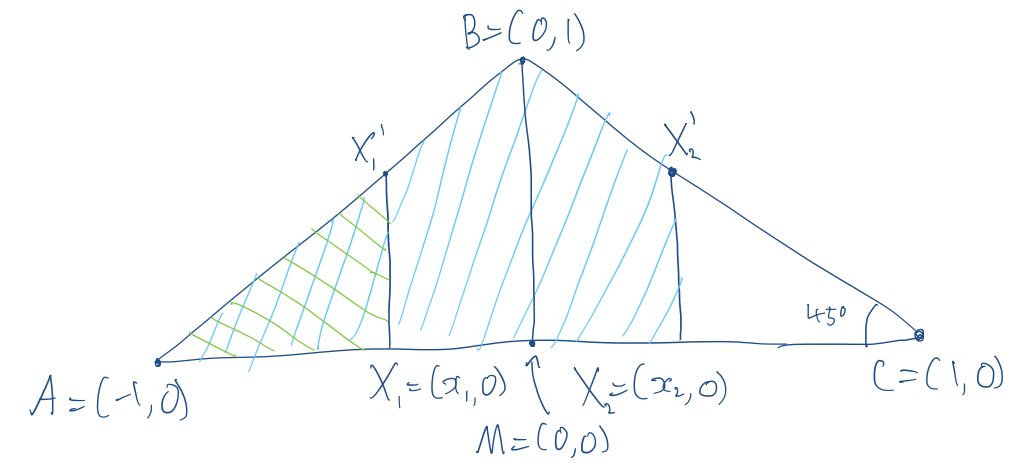
\includegraphics[width=1 \textwidth]{Q2c X diagram.png}
	\caption{Geometric rendering of $D$ showing the cases of $F_\X$}
	\label{fig:q2c-x}
\end{figure}

\begin{multicols}{2}
We know
\begin{align*}
F_\X(-1) &= 0 \\
F_\X(1) &= 1
\end{align*}

\begin{align*}
F_\X(x < -1) &= 0 \\
F_\X(x > 1) &= 1
\end{align*}
\end{multicols}

Case 1: $-1 \leq x \leq 0$.
This implies $F_\X$ is the area of $\triangle\mathrm{A X_{1}^{\prime} X_1}$.
Let $\mathrm{AX_1} = x_1 = \mathrm{X_1 X'_1}$, which implies $x_1 = x + 1$:

\begin{align*}
\mathrm{Area(AX_1'X_1)} &= \frac{1}{2}bh \\
&= \frac{1}{2}x_1^2 \\
\end{align*}

Therefore
\[
F_\X(-1 \leq x \leq 0) = \frac{1}{2}(x + 1)^2
\]

Case 2: $0 < x \leq 1$.
This implies $F_\X(x)$ is the area of $\mathrm{ABX'_2X_2}$.
Note $x = MX_2$, and that $X_2X'_2 = X_2C$

\begin{align*}
\Area{\mathrm{ABX'_2X_2}} &= \Area{\triangle\mathrm{ABM}} + \Area{\mathrm{MBX_2'X_2}} \\
\Area{\triangle ABM} &= \frac{1}{2} \\
\Area{MBX'_2X_2} &= \Area{MBC} - \Area{X_2X_2'C} \\
\Area{MBC} &= \Area{ABM} = \frac{1}{2} \\
\Area{X_2X_2'C} &= \frac{1}{2}bh \\
&= \frac{1}{2} \cdot (1 - x) \cdot (1 - x) \\
&= \frac{1}{2}(1-x)^2 \\
\end{align*}

This is enough information to express $F_\X$:

\begin{align*}
\implies F_\X(0 < x \leq 1) &= (\frac{1}{2}) + (\frac{1}{2} - \frac{1}{2}(1 - x)^2) \\
&= 1 - \frac{1}{2}(1 - 2x + x^2) \\
&= 1 - \frac{1}{2} + x - \frac{1}{2}x^2 \\
&= -\frac{1}{2}x^2 + x + \frac{1}{2}
\end{align*}

Combining cases:

\begin{align*}
\therefore F_\X =
\begin{cases}
0 &: x < -1 \\
\frac{1}{2}(1 + x)^2 &: -1 \leq x \leq 0 \\
-\frac{1}{2}x^2 + x + \frac{1}{2} &: 0 < x \leq 1 \\
1 &: x > 1
\end{cases}
\end{align*}
